\chapter{The semantic preservation theorem and its dependencies}
\label{app:tree-beh-pres-thm}

\begin{figure}[H]
  \centering
  \resizebox{\textwidth}{!}{%
    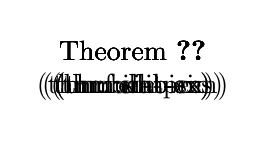
\begin{tikzpicture}
      \tikzset{level distance=200pt}
      \Tree [.\node {
        \begin{tabular}{@{}c@{}}
          Theorem~\ref{thm:beh-pres} \\
          (\nameref{thm:beh-pres}) \\
        \end{tabular}
      };
      [.\node {
        \begin{tabular}{@{}c@{}}
          Theorem~\ref{thm:elab-ex} \\
          (\nameref{thm:elab-ex}) \\
        \end{tabular}
      }; ]
      [.\node {
        \begin{tabular}{@{}c@{}}
          Theorem~\ref{thm:init-ex} \\
          (\nameref{thm:init-ex}) \\
        \end{tabular}
      }; ]
      [.\node {
        \begin{tabular}{@{}c@{}}
          Theorem~\ref{thm:sim-ex} \\
          (\nameref{thm:sim-ex}) \\
        \end{tabular}
      }; ]
      [.\node {
        \begin{tabular}{@{}c@{}}
          Theorem~\ref{thm:full-bisim} \\
          (\nameref{thm:full-bisim}) \\
        \end{tabular}
      }; ]
      ]
    \end{tikzpicture}
  }
\end{figure}
\begin{figure}[H]
  \centering
  \resizebox{\textwidth}{!}{%
    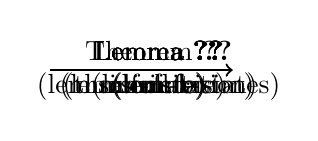
\begin{tikzpicture}[sibling distance=40pt]
      \tikzset{level distance=200pt}
      \Tree [.\node {
        \begin{tabular}{@{}c@{}}
          Theorem~\ref{thm:full-bisim} \\
          (\nameref{thm:full-bisim}) \\
        \end{tabular}
      };
      [.\node {
        \begin{tabular}{@{}c@{}}
          Lemma~\ref{lem:sim-init-states} \\
          (\nameref{lem:sim-init-states}) \\
        \end{tabular}
      }; ]
      [.\node {
        \begin{tabular}{@{}c@{}}
          Lemma~\ref{lem:fst-re} \\
          (\nameref{lem:fst-re}) \\
        \end{tabular}
      }; ]
      [.\node(thmfe) {
        \begin{tabular}{@{}c@{}}
          Lemma~\ref{lem:fe} \\
          (\nameref{lem:fe}) \\
        \end{tabular}
      }; ]
      [.\node(thmsim) {
        {\begin{tabular}{@{}c@{}}
          Lemma~\ref{lem:simulation} \\
          (\nameref{lem:simulation}) \\
         \end{tabular}}
      };
      \node {{\begin{tabular}{@{}c@{}}
          Lemma~\ref{lem:re} \\
          (\nameref{lem:re}) \\
         \end{tabular}}}; ] ]

      \draw (thmsim.west) edge[thick, ->] (thmfe.east);
    \end{tikzpicture}
  }
\end{figure}

\begin{figure}[H]
  \centering
  \resizebox{\textwidth}{!}{%
    
\begin{tikzpicture}[scale=.5, sibling distance=40pt]
      \tikzset{level distance=400pt}
      \tikzset{grow'=right}
      \tikzset{execute at begin node=\strut}
      \tikzset{every tree node/.style={anchor=base west}}
      
      \Tree [.\node {
        \begin{tabular}{@{}c@{}}
          Lemma~\ref{lem:re} \\
          {\fontsize{30}{33}\selectfont (\nameref{lem:re}) } \\
        \end{tabular}
      };
      [.\node {
        \begin{tabular}{@{}c@{}}
          Lemma~\ref{lem:re-equal-marking} \\
          \fontsize{30}{33}\selectfont  (\nameref{lem:re-equal-marking}) \\
        \end{tabular}
      }; ]
      [.\node {
        \begin{tabular}{@{}c@{}}
          Lemma~\ref{lem:re-equal-tc} \\
          \fontsize{30}{33}\selectfont (\nameref{lem:re-equal-tc}) \\
        \end{tabular}
      }; ]
      [.\node {
        \begin{tabular}{@{}c@{}}
          Lemma~\ref{lem:re-equal-reset-orders} \\
          \fontsize{30}{33}\selectfont (\nameref{lem:re-equal-reset-orders}) \\
        \end{tabular}
      }; ]
      [.\node(thmsim) {
        {\begin{tabular}{@{}c@{}}
           Lemma~\ref{lem:re-equal-action-exec} \\
           \fontsize{30}{33}\selectfont (\nameref{lem:re-equal-action-exec}) \\
         \end{tabular}}
     }; ]
     [.\node {
       \begin{tabular}{@{}c@{}}
         Lemma~\ref{lem:re-equal-fun-exec} \\
         \fontsize{30}{33}\selectfont (\nameref{lem:re-equal-fun-exec}) \\
       \end{tabular}
     }; ]
     [.\node {
       \begin{tabular}{@{}c@{}}
         Lemma~\ref{lem:re-equal-sens} \\
         \fontsize{30}{33}\selectfont (\nameref{lem:re-equal-sens}) \\
       \end{tabular}
     }; ]
     [.\node {
      \begin{tabular}{@{}c@{}}
         Lemma~\ref{lem:re-equal-not-sens} \\
         \fontsize{30}{33}\selectfont (\nameref{lem:re-equal-not-sens}) \\
      \end{tabular}
    }; ]
    [.\node {
      \begin{tabular}{@{}c@{}}
         Lemma~\ref{lem:re-equal-cond-comb} \\
         \fontsize{30}{33}\selectfont (\nameref{lem:re-equal-cond-comb}) \\
      \end{tabular}
    }; ]
    [.\node {
      \begin{tabular}{@{}c@{}}
         Lemma~\ref{lem:re-equal-cond} \\
         \fontsize{30}{33}\selectfont (\nameref{lem:re-equal-cond}) \\
      \end{tabular}
    }; ] ]

  \end{tikzpicture}
}
\end{figure}


\begin{figure}[H]
  \centering
  \resizebox{\textwidth}{!}{%
    
\begin{tikzpicture}[scale=.5, sibling distance=30pt]
      \tikzset{level distance=400pt}
      \tikzset{grow'=right}
      \tikzset{execute at begin node=\strut}
      \tikzset{every tree node/.style={anchor=base west}}
      
      \Tree [.\node {
        \begin{tabular}{@{}c@{}}
          Lemma~\ref{lem:fe} \\
          {\fontsize{30}{33}\selectfont (\nameref{lem:fe}) } \\
        \end{tabular}
      };
      [.\node {
        \begin{tabular}{@{}c@{}}
          Lemma~\ref{lem:fe-equal-marking} \\
          \fontsize{30}{33}\selectfont  (\nameref{lem:fe-equal-marking}) \\
        \end{tabular}
      }; ]
      [.\node {
        \begin{tabular}{@{}c@{}}
          Lemma~\ref{lem:fe-equal-tc} \\
          \fontsize{30}{33}\selectfont (\nameref{lem:fe-equal-tc}) \\
        \end{tabular}
      }; ]
      [.\node {
        \begin{tabular}{@{}c@{}}
          Lemma~\ref{lem:fe-equal-cond-values} \\
          \fontsize{30}{33}\selectfont (\nameref{lem:fe-equal-cond-values}) \\
        \end{tabular}
      }; ]
      [.\node(thmsim) {
        {\begin{tabular}{@{}c@{}}
           Lemma~\ref{lem:fe-equal-act-exec} \\
           \fontsize{30}{33}\selectfont (\nameref{lem:fe-equal-act-exec}) \\
         \end{tabular}}
     }; ]
     [.\node {
       \begin{tabular}{@{}c@{}}
         Lemma~\ref{lem:fe-equal-fun-exec} \\
         \fontsize{30}{33}\selectfont (\nameref{lem:fe-equal-fun-exec}) \\
       \end{tabular}
     }; ]
     [.\node {
       \begin{tabular}{@{}c@{}}
         Lemma~\ref{lem:fe-equal-firable} \\
         \fontsize{30}{33}\selectfont (\nameref{lem:fe-equal-firable}) \\
       \end{tabular}
     }; ]
     [.\node {
      \begin{tabular}{@{}c@{}}
         Lemma~\ref{lem:fe-equal-not-firable} \\
         \fontsize{30}{33}\selectfont (\nameref{lem:fe-equal-not-firable}) \\
      \end{tabular}
    }; ]
    [.\node {
      \begin{tabular}{@{}c@{}}
         Lemma~\ref{lem:fe-equal-fired} \\
         \fontsize{30}{33}\selectfont (\nameref{lem:fe-equal-fired}) \\
      \end{tabular}
    }; ]
    [.\node {
      \begin{tabular}{@{}c@{}}
         Lemma~\ref{lem:fe-equal-not-fired} \\
         \fontsize{30}{33}\selectfont (\nameref{lem:fe-equal-not-fired}) \\
      \end{tabular}
    }; ]
    [.\node {
      \begin{tabular}{@{}c@{}}
         Lemma~\ref{lem:fe-equal-ots} \\
         \fontsize{30}{33}\selectfont (\nameref{lem:fe-equal-ots}) \\
      \end{tabular}
    }; ]
    [.\node {
      \begin{tabular}{@{}c@{}}
         Lemma~\ref{lem:fe-equal-its} \\
         \fontsize{30}{33}\selectfont (\nameref{lem:fe-equal-its}) \\
      \end{tabular}
    }; ] ]

  \end{tikzpicture}
}
\end{figure}

%%% Local Variables:
%%% mode: latex
%%% TeX-master: "../main"
%%% End:
